\documentclass[../notes.tex]{subfiles}
\begin{document}
\section{Day 24}
\subsection{Introduction to Simplicial Homology}
\begin{itemize}
    \item We've learned that $\pi_1(X)$ is one way to measure the ``number of holes'' in $X$.
    \item \underline{Advantages:}
        \begin{enumerate}
            \item Not too hard to visualize
            \item Some computational tools
        \end{enumerate}
    \item \underline{Disdvantages:}
        \begin{enumerate}
            \item Nonabelian group means that it is algebraically weird.
            \item Can't detect ``higher dimensional holes'',
                (e.g.$\pi_1(S^2)=\{1\}$).
        \end{enumerate}
    \item Homology is an attempt to remediate these two issues, and provides
        a different methodology for measuring the number of holes:
        \begin{itemize}
            \item $\oplus$ is an abelian group
            \item $\oplus$ can detect holes of different dimensions
            \item $\oplus$ has good computational holes
            \item $\ominus$ has a what Dr. Clader thinks is a 
                ``super non-intuitive definition''
        \end{itemize}
    \item There are several variants of homology, and we're gonna start with the
        simplicial one. It's simplices, the simplest thing there is. This
        is called the \underline{simplicial homology}.
\end{itemize}
\subsubsection{Simplices, the simplest things that exist}
\begin{definition}
    A set of points, $\{p_0,p_1,p_2,\dots,p_n\}\subseteq \R^N$ is
    \underline{affinely independent} or \underline{geometrically independent}
    if 
    \[
        \{p_1-p_0,\dots,p_n-p_0\}\subseteq \R^N
    \]
    is a linearly independent set of vectors.
\end{definition}
\newpage
\begin{itemize}
    \item \underline{Ex:}\\
        \begin{center}
            \begin{tikzpicture}
                \begin{axis}[
                    xmin=-1, xmax=3,
                    ymin=-1, ymax=3,
                    ]
                    \addplot [color=blue,only marks,mark=*] coordinates { (0,0) (1,0) (0,1) };
                \end{axis}
            \end{tikzpicture}\\
        \end{center}
        \[
            \{(0,0), (1,0), (0,1)\}\subseteq\R^2
        \]
        is affinely independent.\\
    \item \underline{Ex:}\\
        \begin{center}
            \begin{tikzpicture}
                \begin{axis}[
                    xmin=0, xmax=4,
                    ymin=0, ymax=4,
                    ]
                    \addplot [color=blue,only marks,mark=*] coordinates { (1,2) (2,2)  (1,3) };
                \end{axis}
            \end{tikzpicture}\\
        \end{center}
        \[
            \{(1,2), (2,2), (1,3)\}\subseteq\R^2
        \]\\
        That's affine independent set of vectors.\\
        (it's affinely independent)
    \item More generally, if we apply any invertible linear transformation, for example
        translation, rotation, to $\{(0,0),(1,0),(0,1)\}$, the result is affinely 
        independent.
    \item \underline{Ex:}\\
        \begin{center}
            \begin{tikzpicture}
                \begin{axis}[
                    xmin=-2, xmax=6,
                    ymin=-2, ymax=6,
                    ]
                    \addplot [color=blue,only marks,mark=*] coordinates { (0,2) (-1,2) (0,5) };
                \end{axis}
            \end{tikzpicture}\\
        \end{center}
        \[
            \{(0,2), (-1,2), (0,5)\}\subseteq\R^2
        \]\\
    \item \underline{Non-Ex:}
        \begin{center}
            \begin{tikzpicture}
                \begin{axis}[
                    xmin=-1, xmax=3,
                    ymin=-1, ymax=3,
                    ]
                    \addplot [color=blue,only marks,mark=*] coordinates { (0,0) (1,0) (2,0) };
                \end{axis}
            \end{tikzpicture}\\
        \end{center}
        \[
            \{(0,0), (1,0), (2,0)\}\subseteq\R^2
        \]\\
        \newpage
    \item \underline{Non-Ex:}\\
        \begin{center}
            \begin{tikzpicture}
                \begin{axis}[
                        xmin=-1, xmax=3,
                        ymin=-1, ymax=3,
                        ]
                        \addplot [color=blue,only marks,mark=*] coordinates { (0,0) (1,0) (0,1) (1,1) };
                    \end{axis}
                \end{tikzpicture}\\
            \end{center}
        \[
            \{(0,0), (1,0), (0,1), (1,1)\}\subseteq\R^2
        \]
\end{itemize}
\begin{definition}
    Let $\{p_0,p_1,\dots,p_n\}\subseteq \R^N$  be an affinely independent set.
    Then the \underline{simplex} spanned by $\{p_0,p_1,\dots,p_n\}$ is:
    \[
        \sigma=\{a_0p_0+a_1p_1+\dots+a_np_n| a_i\in R^{\geq 0} \forall i,\
        \sum_{0}^{n}a_i=1\}
    \]
    Additionally, we could consider this to be the convex hull of $p_0,\dots,p_n$. We
    say that $\sigma$ is a simplex of \underline{dimension n} or an \underline{n-simplex}
\end{definition}
\begin{itemize}
    \item\underline{Ex:} $(n=0)$\\
        $\{p_0\}$ is affinely indpendent for all $p_0\in \R^N$, then the 0-simplex spanned by
        $\{p_0\}$ is,
        \[
            \sigma = \{a_0p_0| a_0\in R^{\geq 0},\ a_0=1\}=\{p_0\}
        \]
        It's just the point $p_0$
        \newpage
    \item\underline{Ex:} $(n=1)$\\
        $\{p_0,p_1\}$ is affinely independent as long as $p_0\neq p_1$. The
        1-simplex spanned by $\{p_0,p_1\}$ is:
        \[
            \sigma = \{a_0p_0+a_1p_1| a_0,a_1\in R^{\geq 0},\ a_0+a_1=1\}
        \]
        With $p_0=(0,1)$, $p_1=(1,2)$, we have\\
        \begin{center}
        \begin{tikzpicture}
            \begin{axis}[
                xmin=-1, xmax=3,
                ymin=-1, ymax=3,
                ]
                \addplot [color=blue,mark=*] coordinates { (0,1)(1,2)};
            \end{axis}
        \end{tikzpicture}\\
    \end{center}
    \item\underline{Ex:} $(n=2)$\\
        E.g.
        \[ \sigma=\{a_0(0,0)+a_1(1,0)+a_2(0,1), (1,1)| 
            a_0,a_1,a_2\in R^{\geq 0},\ a_0+a_1+a_2=1\}
        \]
        However, since $p_0=(0,0)$, this is jut,
        \[
            \sigma=\{a_1(1,0)+a_2(0,1), (1,1)| 
            a_1,a_2\in R^{\geq 0},\ a_1+a_2\leq1\}
        \]
        \begin{center}
            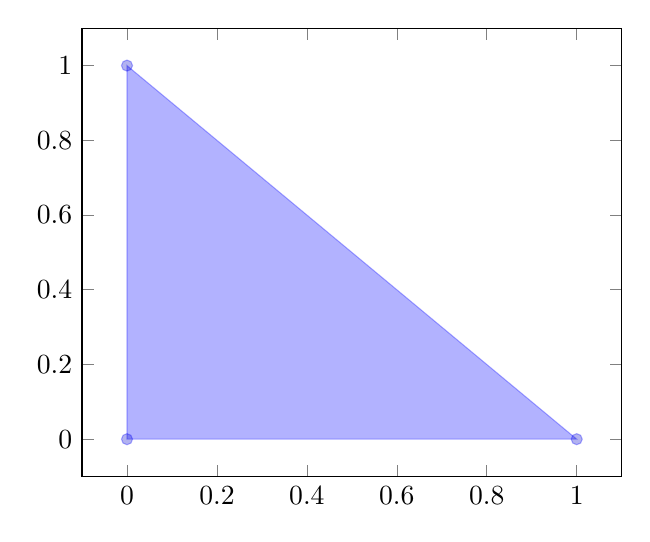
\begin{tikzpicture}
                \begin{axis}
                    \addplot+[fill, opacity=0.3] coordinates 
                    { (0,0) (1,0) (0,1) } --cycle;
                \end{axis}
            \end{tikzpicture}\\
        \end{center}
    \item \underline{Fact:} More generally:
        \begin{itemize}
            \item The 2-simplex spanned by $\{p_0,p_1,p_2\}\subseteq\R^N$ is a triangle
                with $p_0,p_1,p_2$ as vertices.
            \item The 3-simplex spanned by $\{p_0,p_1,p_2,p_3\}\subseteq\R^N$ is a 
                tetrahedron with $p_0,p_1,p_2,p_3$ as vertices.
        \end{itemize}
    \item \underline{Ex:}
        \filled{(0,0) (1,0) (-1,1)}
        \[
            \{(0,0), (1,0), (-1,1)\}
        \]\\
        is affinely independent, and also a simplex.
\end{itemize}
\begin{definition}
    Let $\sigma$ be a simplex spanned by $\{p_0,\dots,p_n\}$. Then a \underline{face}
    of $\sigma$ is any simplex spanned by a nonempty subset of $\sigma$
\end{definition}
\begin{itemize}
    \item \underline{Ex:}
        \[
            \sigma = \text{3-simplex spanned by $\{(0,0,0), (1,0,0), (0,1,0), (0,0,1)\}$}
        \]
        \begin{center}
            \begin{tikzpicture}[line join=bevel,z=2.5, y=2]
                \begin{axis}[
                    y dir = reverse,
                    xmin=0,xmax=1,
                    ymin=0,ymax=1,
                    zmin=0,zmax=1
                    ]
                    \addplot3+[fill,
                               fill opacity=.3,
                               fill color=blue]
                    coordinates {
                        (0,0,1)
                        (1,0,0)
                        (0,1,0)
                    } --cycle;
                    \addplot3+[black, line style=dashed]
                    coordinates {
                        (0,0,0)
                        (1,0,0)
                        (0,1,0)
                    } --cycle;
                    \addplot3+[black, line style=dashed]
                    coordinates {
                        (0,0,0)
                        (1,0,0)
                        (0,0,1)
                    } --cycle;
                    \addplot3+[black, line style=dashed]
                    coordinates {
                        (0,0,0)
                        (0,0,1)
                        (0,1,0)
                    } --cycle;
                \end{axis}
            \end{tikzpicture}
        \end{center}
        \underline{Faces:}\\
        \begin{itemize}
            \item Each vertex (spanned by a 1-element subset)
            \item Each edge, (spanned by 2-element subsets)
            \item Each surface, (spanned by 3-element subsets)
            \item The whole thing, (spanned by 4-element subsets)
        \end{itemize}
\end{itemize}
\end{document}
